\documentclass[main.tex]{subfiles}
\begin{document}
\chapter*{Bilag - Kravspecifikation}

\section{Versionshistorik}
\begin{longtabu} to \linewidth{@{}l l l X[l]@{}}
    Version 	&    Dato 		&    Ansvarlig 	&    Beskrivelse\\[-1ex]
    \midrule
    0.1 		&  	21-09-2015 	&   MHNK og MBA 	&   Oprettelse og udfyldning af kravspecifikation \\
	0.2			&	24-09-2015	&	DHC og ABH	&	Omskrivning af UC1 - UC5 \\
	
    
\label{version_Systemark}
\end{longtabu}






\section{Systembeskrivelse}
\subsection{Aktør kontekstdiagram}



\section{Funktionelle krav}
\subsection{Use case diagram}

\begin{figure}[H]
\centering
{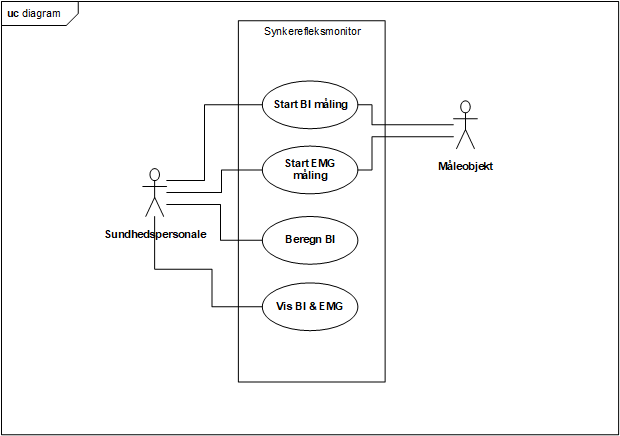
\includegraphics[width=\textwidth]
{Figure/usecasediagram}}
\caption{Use case diagram}
\label{Use case diagram}
\end{figure}

\subsection{Use cases - fully dressed}

\begin{longtabu} to \linewidth{@{}l r X[l]@{}} %UC1%
	{\large \textbf{Use Case 1}} && \\
	\toprule
	Scenarie 				&&	Hovedscenarie\\
	Navn 					&& 	Start BI måling\\
	Mål 					&& 	At få foretaget en BI måling\\
	Initiering 				&& 	Startes af Sundhedspersonale\\
	Aktører 				&& 	Sundhedspersonale (primær), Måleobjekt (sekundær)\\
	Referencer 				&& 	\\
	Samtidige forekomster  	&& 	En BI måling pr. kørsel \\
	Forudsætninger 			&&	Alle systemer er ledige og operationelle. Elektroder påsat måleobjekt\\ 
	Resultat 				&& 	BI måling er blevet foretaget efter ønske\\ \midrule
	Hovedscenarie 			&    1. 	&	GUI vindue er åben\\				 	
							&    2. 	& 	Sundhedspersonale trykker på Start BI måling-knap\\ 
							& 	 3.		&	 Systemet foretager målingen indtil der trykkes på Stop måling-knap \\[-1ex]
                            & 	 4.		&	 Systemet har gemt måling i en fil \\[-1ex]
	Undtagelser 			&			& 	-  \\ \bottomrule
	
	\caption{Fully dressed Use Case 1}
	\label{UC1}
\end{longtabu}

\begin{longtabu} to \linewidth{@{}l r X[l]@{}} %UC1%
	{\large \textbf{Use Case 2}} && \\
	\toprule
	Scenarie 				&&	Hovedscenarie\\
	Navn 					&& 	Start EMG måling\\
	Mål 					&& 	At få foretaget en EMG måling\\
	Initiering 				&& 	Startes af Sundhedspersonale\\
	Aktører 				&& 	Sundhedspersonale (primær), Måleobjekt (sekundær)\\
	Referencer 				&& 	\\
	Samtidige forekomster  	&& 	En EMG måling pr. kørsel \\
	Forudsætninger 			&&	Alle systemer er ledige og operationelle. Elektroder påsat måleobjekt\\ 
	Resultat 				&& 	EMG måling er blevet foretaget efter ønske\\ \midrule
	Hovedscenarie 			&    1. 	&	GUI vindue er åben\\				 	
							&    2. 	& 	Sundhedspersonale trykker på Start EMG måling-knap\\ 
							& 	 3.		&	 Systemet foretager målingen indtil der trykkes på Stop måling-knap \\[-1ex]
                            & 	 4.		&	 Systemet har gemt måling i en fil \\[-1ex]
	Undtagelser 			&			& 	-  \\ \bottomrule
	
	\caption{Fully dressed Use Case 2}
	\label{UC2}
\end{longtabu}

\begin{longtabu} to \linewidth{@{}l r X[l]@{}} %UC1%
	{\large \textbf{Use Case 3}} && \\
	\toprule
	Scenarie 				&&	Hovedscenarie\\
	Navn 					&& 	Beregn BI\\
	Mål 					&& 	At få beregent BI\\
	Initiering 				&& 	Startes af Sundhedspersonale\\
	Aktører 				&& 	Sundhedspersonale (primær)\\
	Referencer 				&& 	Use case 1\\
	Samtidige forekomster  	&& 	En BI beregning pr. kørsel \\
	Forudsætninger 			&&	Use case 1 er foretaget\\ 
	Resultat 				&& 	BI beregning er foretaget efter ønske\\ \midrule
	Hovedscenarie 			&    1. 	&	Sundhedspersonale trykker på Beregn BI-knap\\	
							&    2. 	& 	Systemet foretager BI beregning\\ 
							& 	 3.		&	Systemet har gemt BI beregning \\[-1ex]
    Undtagelser 			&			& 	-  \\ \bottomrule
	
	\caption{Fully dressed Use Case 3}
	\label{UC3}
\end{longtabu}

\begin{longtabu} to \linewidth{@{}l r X[l]@{}} %UC1%
	{\large \textbf{Use Case 4}} && \\
	\toprule
	Scenarie 				&&	Hovedscenarie\\
	Navn 					&& 	Vis BI \& EMG\\
	Mål 					&& 	At få vist BI \& EMG måling over tid på en graf\\
	Initiering 				&& 	Startes af Sundhedspersonale\\
	Aktører 				&& 	Sundhedspersonale (primær)\\
	Referencer 				&& 	\\
	Samtidige forekomster  	&& 	En graf pr. kørsel \\
	Forudsætninger 			&&	Use case 1, 2 og 3 er foretaget\\ 
	Resultat 				&& 	Grafen er vist efter ønske\\ \midrule
	Hovedscenarie 			&    1. 	&	Sundhedspersonale trykker på Vis BI \& EMG-knap\\				 	
							&    2. 	& 	Grafen vises i GUI vinduet\\
	Undtagelser 			&			& 	-  \\ \bottomrule
	
	\caption{Fully dressed Use Case 4}
	\label{UC4}
\end{longtabu}


\section{Ikke-funktionelle krav}
\subsection{(F)URPS+}

\textbf{Functionality}
\begin{enumerate}
\item Synkerefleksmonitor skal indeholde en BI Start Måling-knap til at igangsætte Bi målingerne
\item Synkerefleksmonitor skal indeholde en EMG Start Måling-knap til at igangsætte EMG målingerne 
\item Synkerefleksmonitor skal indeholde en Stop Måling-knap, hvorfra måling kan stoppes
\item Synkerefleksmonitor skal indeholde en Vis BI \& EMG-knap, hvorfra grafen vises
\item Synkerefleksmonitor skal indeholde en Beregn BI-knap, hvorfra den beregnet BI gemmes
\end{enumerate}

\textbf{Usability}
\begin{enumerate}
\item Sundhedspersonalet skal kunne starte en BI-måling maksimalt 30 sekunder efter systemet er startet
\item Sundhedspersonalet skal kunne starte en EMG-måling maksimalt 30 sekunder efter systemet er startet
\item Sundhedspersonalet skal kunne se grafen maksimalt 10 sekunder efter tryk på Vis Bi \& EMG-knap
\item Sundhedspersonalet skal kunne beregne BI maksimalt 10 sekunder efter tryk på Beregn BI-knap
\end{enumerate}
                                                                                                
\textbf{Reliability}
\begin{enumerate}
\item Det skal maksimalt tage 5 timer at gendanne systemet (MTTR - Mean Time To Restore)
\item Systemet skal have en oppetid uden nedbrud på minimum 1 måned (720 timer) (MTBF - Mean Time Between Failure)   
\item Systemet skal have en oppetid/køretid på: 
\end{enumerate}

%\begin{ceqn}
%\begin{equation}
%Availability = \frac{MTBF}{MTBF+MTTR}\cdot100 = \frac{720}{720+5}\cdot100 = 99,31 \%
%\end{equation}
%\end{ceqn}
					
\textbf{Performance}
\begin{enumerate}
\item Blodtryksmåleren skal, indenfor 3 sekunder, kunne vise systolisk og diastolisk blodtryk via grafen. Dette accepteres med en tolerance på +/- 15 \%
\item Blodtryksmåleren skal, indenfor 5 sekunder fra der er trykket på Stop Gem-knap, have gemt målingerne i Databasen. Dette accepteres med en tolerance på +/- 15 \%
\item Grafen vises i ét vindue, hvor y-aksen måles i mmHg (millimeter kviksølv) og x-aksen i tid pr. sekund
\item Hvert 3. sekund skal værdier for systolisk og diastolisk blodtryk, samt puls opdateres. Dette accepteres med en tolerance på +/- 15 \%
\item Grafen for blodtryk skal køre kontinuerligt i GUI efter følgende princip (figur \ref{fig:Graf for blodtryks visning}), hvor det blå signal erstatter det orange signal ved, at den seneste måling altid sættes ved cursorens placering


\item Når der trykkes på Stop Gem-knap gemmes signals rådata under det indtastede Forsøgsnavn og et autogenereret Id. \textit{"Forsøgsnavn\_Id"}
\item Systemet skal kunne måle blodtryksværdier fra 0 til 250 mmHg
\end{enumerate}


\textbf{Supportability}
\begin{enumerate}
\item Forskeren skal kunne udskifte batterierne til hardwaren inden for 2 minutter 
\item Softwaren skal opbygges med lav kobling
\end{enumerate}





\end{document}